
%%%%%%%%%%%%%%%%%%%%%%%%%%%%%%%%%%%%%%%%%%%%%%%%%%%%%%%%%%%%%%%%%%%%%%%%%%%%%
\section{Code tests}
\label{sec.tests}

Ensuring that a complex piece of software is behaving correctly is a
non-trivial task.  While there are a range of techniques that one can
apply to ensure correctness, the \enzo\ code uses two primary methods:
a suite of test problems that can be compared to previous versions of
the code, to ensure that \enzo\ is, e.g., running correctly on a new
computer, with a new compiler, or after substantial changes have been
made to the code base; and by direct comparisons to other
astrophysical fluid dynamics codes.  We describe the \enzo\ test
methodology in Section~\ref{sec.tests.suite}, code comparisons in
Section~\ref{sec.tests.compare}, and show a small set of
representative test problems in Section~\ref{sec.tests.problems}.  We
further note that the \enzo\ test suite
(Section~\ref{sec.tests.suite}) contains hundreds of test problems, as
well as the ability to compare to a ``gold standard'' solution, and
thus all of the tests shown here are easily reproducible by the
reader.

%%%%%%%%%%%%%%%%%%%%%%%%%%%%%%%%%%%%%%%%%%%%%%%%%%%%%%%%%%%%%%%%%%%%%%%%%%%%%
\subsection{Verifying and validating the \enzo\ code}
\label{sec.tests.vandv}

\subsubsection{The \enzo\ test suite}
\label{sec.tests.suite}

\enzo\ is capable of simulating a large variety of problems types, with
all but a small few requiring only a parameter file as sole input.
The notable exception is the cosmology simulation, which takes as
input initial conditions created by other codes.  These test problems
span a wide range in complexity.  At one end of this spectrum are
simple problems that utilize only a single component of \enzo\ and for
which analytic solutions exist for comparison with the simulation
results.  At the opposite end are problems that exercise a large
portion of \enzo's machinery in concert.  Together, the available
problem types fully cover all of \enzo's functionality.  This enables
them to serve as a vehicle for verifying that the code's behavior
remains stable over time.

\enzo\ uses an automated testing framework that allows a user to run,
with a single command, a set of test problems and compare the results
against results produced by any other version of the code.  Within the
\enzo\ source distribution, the test problem parameter files are stored
in a nested directory structure organized according to the primary
functionality tested, e.g., hydrodynamics, gravity, cooling, etc.
Each parameter file is accompanied by a text file containing various
descriptive keywords, such as the machinery tested, the
dimensionality, and the approximate run time.  A test runner script is
responsible for taking as input from the user a series of keywords
with which to select a subset of all available test problems.  The
test problems are also grouped into three suites: the quick, push, and
full suites, each a superset of the ones named before.  The quick
suite is considered to minimally cover the primary functionality in
\enzo\ and is designed to be run repeatedly during the development
process.  The push suite has slightly increased feature coverage and
is mandated to be run before code changes are accepted into the main
repository.  The full suite consists of all test problems which can be
run with no additional input.  Approximate run times for the quick,
push, and full suite are 15 minutes, 1 hour, and 60 hours,
respectively.

After the test problems are selected by the test runner script, they
are run in succession either by with \enzo\ executable contained
within that distribution or an external executable built from another
version and specified by the user.  This allows for any version of the
code to be tested with an identical set of test problems.  After
running the test problem simulations, the test runner then performs a
series of basic analysis tasks using the \texttt{yt} analysis toolkit
\citep{2011ApJS..192....9T, 2011arXiv1112.4482T}.  The default
analysis performed on all test problems includes calculation of
various statistics, such as extrema; mean; and variance, on the fields
present in the output data.  Custom analysis provided by scripts that
accompany the test problem parameter files is run for special cases,
such as when an analytical solution exists that can be compared
against the simulation data.  After the analysis is performed, the
results are compared against a set of gold standard results which are
maintained on a website and downloaded on the fly by the test runner
script.  Alternately, results from any version of \enzo\ can be stored
locally and compared to any other version of the code.  In
Section~\ref{sec.tests.problems}, we describe some of the key test
problems which are used to verify proper behavior.  All of these test
problems, as well as the scripts to generate the figures from them,
are available in the \enzo\ test suite.

\subsubsection{Code comparisons}
\label{sec.tests.compare}

Over the course of its existence, \enzo\ has been involved in several
comparisons with other astrophysical codes used for self-gravitating
fluid dynamics.  In general, \enzo\ behaves in a manner similar to other
grid-based (and particularly AMR-based) codes, as we will summarize below.

\enzo\ has been involved in several cosmological code comparisons,
including the Santa Barbara Cluster code comparison project
\citep{SantaBarbara}, a large comparison of N-body simulations
\citep{2008CS&D....1a5003H}, as well as several direct comparisons
between \enzo\ and the GADGET SPH code under a variety of
circumstances, including N-body and adiabatic hydrodynamics
\citep{2005ApJS..160....1O,2005MNRAS.364..909V, 2011MNRAS.418..960V}
and simulations of the Lyman-alpha forest \citep{2007MNRAS.374..196R}.
The \enzo\ code typically has a more difficult time resolving
small-scale self-gravitating structures (for an equivalent dark matter
particle count and nominally equivalent force resolution), but does
comparably well as a tree-based code for larger structure, and is
typically superior in terms of resolving fluid features due to its
higher-order (and artificial viscosity-free) hydrodynamics solver.
When examining classical test cases such as the Santa Barbara
project \citep{SantaBarbara}, \enzo\ forms galaxy clusters with very similar density,
temperature, and entropy profiles to other grid-based codes that use
Godunov-type hydro methods, which
systematically differ from particle-based codes using SPH.  Similarly,
in galaxy cluster simulations that look specifically at the properties
of cosmological shocks \citep[e.g.][]{2011MNRAS.418..960V}, \enzo\
produces results that are similar to other high-order grid-based
hydrodynamics codes, and far superior behavior of \enzo\ in
low-density regions when compared to a particle-based code.  In tests
of the Lyman-alpha forest that include radiative cooling and a uniform
metagalactic ultraviolet background, \enzo\ and Gadget provide results
on metrics such as the matter power spectrum that are comparable to
within 5\% \citep{2007MNRAS.374..196R}.

Several comparisons have been made that focus specifically on
hydrodynamics solvers.  In particular, the work of
\citet{2007MNRAS.380..963A} and \citet{Tasker2008} perform
head-to-head comparisons between several grid- and particle-based
codes for a variety of test problems (including shocked gas clouds,
self-gravitating, translating clouds, and Sedov-Taylor explosions),
and show that \enzo\ is comparable or superior in behavior to the
other grid-based hydrodynamics codes involved in the comparison, and
provide useful information on whether an AMR code such as \enzo\
experiences challenges.  More specific comparisons, including one
specifically testing the linear and nonlinear growth of the
Kelvin-Helmholz instability \citep{2012ApJS..201...18M} and one more
broadly examining Galilean invariance in grid-based codes
\citep{2010MNRAS.401.2463R} show that \enzo, and in particular its
implementation of the Piecewise Parabolic Method hydrodynamics solver,
converge to the correct solution as expected, and generally provide
less diffusive solutions than lower-order codes, including those that
use artificial viscosity.  Finally, two code comparison projects have
been undertaken to examine turbulence in hydro codes -- one studied
the behavior of decaying isothermal supersonic turbulence
\citep{2009A&A...508..541K}, and the other looked at supersonic
magnetohydrodynamical turbulence \citep{2011ApJ...737...13K}.  Both
included the \enzo\ code, with the former testing the PPM
hydrodynamics and the latter the constrained transport MHD
implementation.  In both cases, \enzo\ performed similarly to other
grid-based codes that use Godunov-based fluid solvers, and typically
had better effective resolution than particle-based codes using the
same number of particles as the \enzo\ simulation used grid cells.

Three other comparisons between portions of the \enzo\ code and other
simulation tools have been performed in recent years.  The
flux-limited diffusion radiation transport scheme was measured against
several test problems by \citet{IlievEtAl2009}, producing results that
are similar to both expected results and other methods, although there
are some minor differences (although all codes in the study exhibited
differences from the majority of other codes on at least a subset of
the tests).  \citet{2011ApJ...726...55T} shows the result of varied
reaction rate coefficients for the formation of molecular hydrogen via
the 3-body process in both the \enzo\ and Gadget-2 codes.  Similar
trends were visible in both the \enzo\ and Gadget simulations, though
at a nominally equivalent resolution (i.e., with particle and cell gas
masses being comparable) \enzo\ simulations typically displayed a much
higher level of gas structure.  This is unsurprising due to \enzo's
higher-order hydro solver.  Finally, \citet{2012ApJ...744...52P} show
the results of comparing \enzo\ in its non-AMR mode to a
smoothed-particle hydrodynamics code, SNSPH, in the context of
common-envelope binary stellar interactions.  The authors show that
the codes display reasonable convergence properties as a function of
simulation resolution, and also agree quite well with each other --
however, the observed mass-loss rates do not agree particularly well
with observations.

%%%%%%%%%%%%%%%%%%%%%%%%%%%%%%%%%%%%%%%%%%%%%%%%%%%%%%%%%%%%%%%%%%%%%%%%%%%%%
\subsection{Representative test problems}
\label{sec.tests.problems}

General structure for each test problem:  Outline how the test problem is constructed (initial and boundary conditions), 
the analytical solution, why we have in the paper (what does it break, or what flaw does it expose (not in enzo of course)),
a plot showing how well enzo solves said test problem, and a brief description of the plot and how awesome enzo is.

%%%%%%%%%%%%%%%%%%%%%%%%%%%%%%%%%%%%%%%
\subsubsection{Sod Shock Tube}
\label{sec.tests.sodshock}
\red{(Greg)}
Problem type 1.  AMR version.  Tests the hydro.
This is also problem 7.2 in the FLASH method paper.

%%%%%%%%%%%%%%%%%%%%%%%%%%%%%%%%%%%%%%%
\subsubsection{Wave pool}
\label{sec.tests.wavepool}
\red{(Greg)}
Problem type 2, with AMR.  Tests reflections of waves at grid boundaries.

%%%%%%%%%%%%%%%%%%%%%%%%%%%%%%%%%%%%%%%
\subsubsection{Shock pool}
\label{sec.tests.shockpool}
\red{(Greg)}
Problem type 3, with AMR.  Tests passage of shock through a refinement boundary.

%%%%%%%%%%%%%%%%%%%%%%%%%%%%%%%%%%%%%%%
\subsubsection{Double mach reflection}
\label{sec.tests.doublemach}
\red{(Brian)}

The double mach reflection test is a classic two-dimensional test of
hydrodynamic algorithms, and was originally described in
\citet{1984JCoPh..54..115W} \citep[and more recently
in][]{2008ApJS..178..137S}.  In this problem (shown in
Figure~\ref{fig.doublemach}), a shock is injected at an angle to a
reflecting surface, and a jet appears along the reflecting surface.
The ideal solution is self-similar, and the appearance of this
solution is highly sensitive to numerical diffusion.  If numerical
noise is present, a Kelvin-Helmholz instability develops along this
jet and breaks the self-similarity.

In the test problem shown in Figure~\ref{fig.doublemach}, a 2D
simulation with $960 \times 240$ cells was formed with a domain of $x
= [0, 4]$ and $y = [0, 1]$.  We use an ideal gas equation of state of
$\gamma = 1.4$, a pre-shock density of 1.4, and a pre-shock specific
internal energy of $2.5/1.4$ (all in arbitrary units).  A Mach 10
shock is initialized with a shock normal that is 30$^\circ$ from the
x-axis and an initial position on the lower boundary of x$ = 1/6$.
The lower y boundary and right x boundary are reflecting; the left x
boundary is inflowing, and the upper y boundary has a time-dependent
boundary condition that allows the shock to propagate into the domain
as if it extends to infinity.  The simulation starts at t$ = 0$ and
runs until t$ = 0.205$ (arbitrary units), at which point the rightmost
extent of the shock should be at roughly x$ = 3$.  In this run, we use
the direct Eulerian implementation of the piecewise parabolic hydro
method, with diffusion, flattening, and shock steepening all turned
on.

It is instructive to compare Figure~\ref{fig.doublemach} to Figure 9
in~\citet{1984JCoPh..54..115W}.  By the end of the simulation, a dense
jet is apparent at the leading edge of the shock, propagating along
the x-axis.  The shape of this jet is sensitive to numerical
diffusion, and our figure compares favorably to the higher-order
images from Woodward \& Colella.

\begin{figure}
\begin{center}
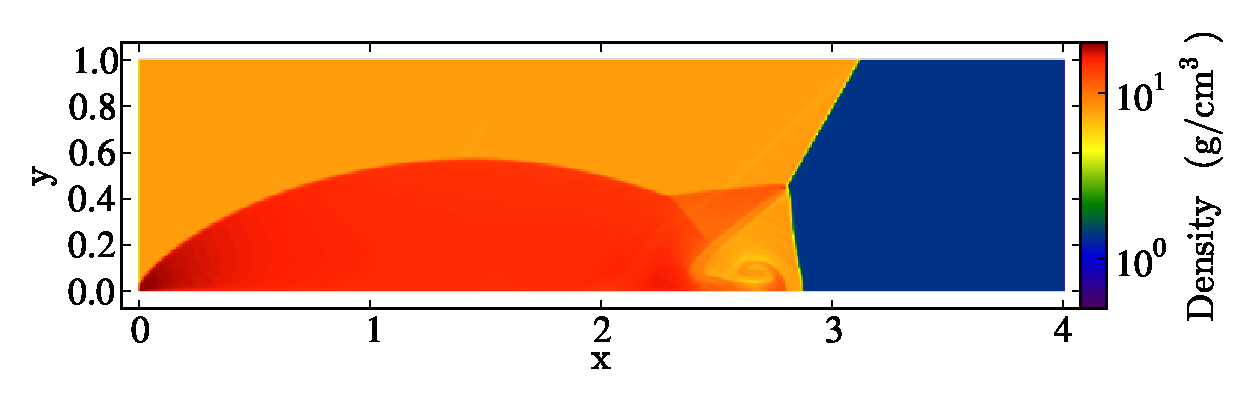
\includegraphics[width=0.8\textwidth]{figures/DoubleMachTest.eps}
\caption{Double mach test.}
\label{fig.doublemach}
\end{center}
\end{figure}

%%%%%%%%%%%%%%%%%%%%%%%%%%%%%%%%%%%%%%%
\subsubsection{Sedov Explosion}
\label{sec.tests.sedov}

\begin{figure}
\begin{center}
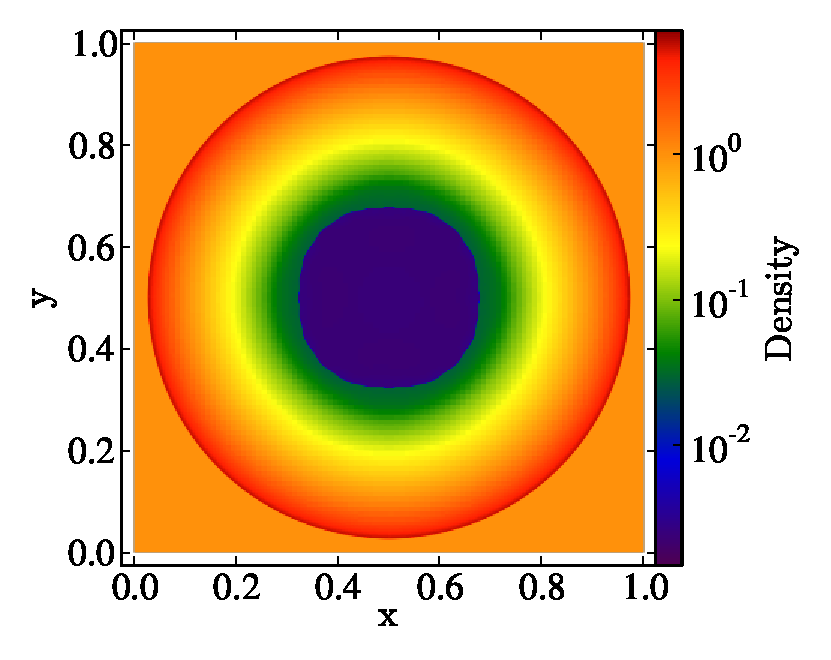
\includegraphics[width=0.4\textwidth]{figures/sedov-ppm-slice.eps}
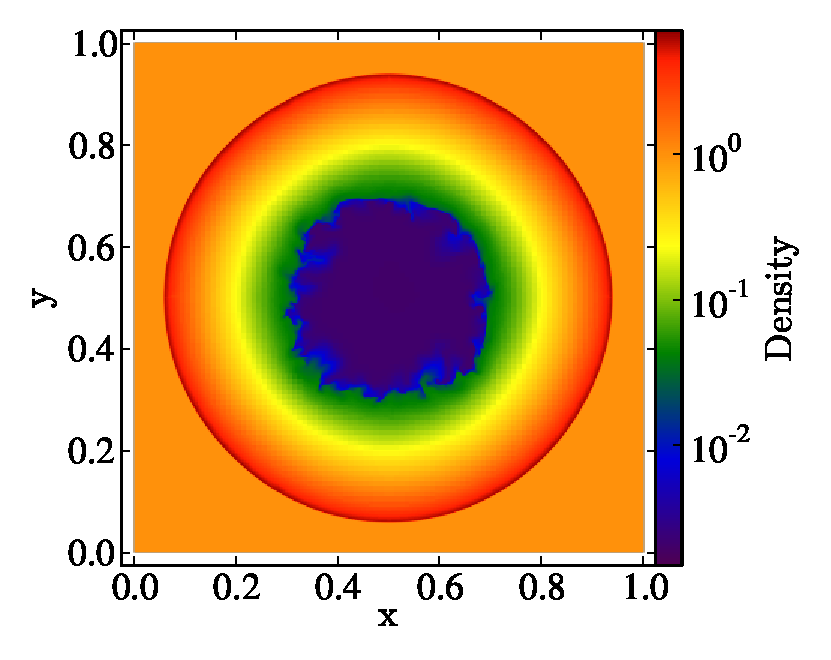
\includegraphics[width=0.4\textwidth]{figures/sedov-zeus-slice.eps}
\caption{Density slice from the Sedov Blast Test at $t =
0.07$. Left-hand image shows the results from PPM ({\tt HydroMethod =
0}), right-hand image shows the results from Zeus ({\tt Hydromethod =
2}). Notably, the Zeus shock front has progressed less far than forthe
PPM run. This is due to energy loss when conserving internal, not
total, energy.}
\label{fig.sedov1}
\end{center}
\end{figure}


\begin{figure}
\begin{center}
\includegraphics[width=\textwidth]{figures/sedov-profiles.eps}
\caption{Radially averaged profiles for the Sedov Blast Test at $t =
0.07$. Clockwise from top-left shows density, velocity, internal
energy and pressure.}
\label{fig.sedov2}
\end{center}
\end{figure}

The Sedov Blast Test \citep{Sedov1959} models an intense explosion,
initiated by depositing thermal energy into a homogenous distribution
of gas. The result is a strong spherical shock wave centered on the
point of energy injection.  This problem is a popular test of
astrophysical numerical codes for three reasons: Firstly, it is
particularly appropriate to astrophysics since it represents the
situation when a supernovae explosion occurs. Secondly, it has an
exact analytical solution whereby the shock front's radial position is
given by:

\begin{equation} r(t) =
\left(\frac{E_0}{\alpha\rho_0}\right)^{1/5}t^{2/5}
\end{equation}

\noindent where $E_0$ is the initial energy injection, $\rho_0$ is the
background density and $\alpha = 1.0$ for cylindrical symmetry and an
ideal gas with $\gamma = 1.4$. For the full derivation see
\citet{Sedov1959}. This solution makes it possible to assess how well
the code performs. Thirdly, the spherical shock is a challenging
problem for numerical codes (both grid and particle) since the shock
wave increases in size as the simulation progresses and its
symmetrical nature highlights any directional preferences that grid
codes can succumb to. The test presented here is the two-dimensional
version that is included in the Enzo distribution. The
three-dimensional results from this test, both for Enzo and three
other leading astrophysics codes, can be founds in \citet{Tasker2008}.

In the initial state, the box contains a homogenous distribution of
gas at a density of 1 (note that, in the absense of gravity, this
problem is scale-free and so without units). Thermal energy is
deposited into a single cell at the center of the box with $E_0 =
10.0$. The problem is completed in two dimensions with reflecting
boundary conditions (the default for Enzo) and uses a boxsize of side
$1$. For this problem, we selected a top grid of $100 \times 100$ and
four levels of refinement, placed based on shock location and the
slope in density and total energy (this corresponds to cell flagging
methods 1 and 3 in the Enzo parameter file). The exception to this
scheme is in the initial conditions where grids are placed directly
around the injection point. The results were assessed at $t = 0.07$,
which corresponding to a time just before the shock reaches the box
edge (see Figure~\ref{fig.sedov1}).

Figure~\ref{fig.sedov2} shows the radial profiles for the simulation
run with the PPM hydro-solver (blue dashed line) and the Zeus
hydro-solver (red dash-dot-dot line) together with the analytical
solution (black solid line). Clockwise from the top-left are density,
velocity, internal energy and pressure. PPM matches the analytical
solution extremely well for all quantities. However, Zeus' shock front
lags behind the analytical position. This can also be seen in the
slices shown in Figure~\ref{fig.sedov1}. The cause of this discrepancy
is that Zeus shows a substantial energy lost during the first few
timesteps and produces a diamond-shaped, rather than spherical,
shockfront during this time. After this, the code correctly conserves
energy but this intial energy loss remains clearly visible in the
position of the shock at $t = 0.07$. This problem was addressed
directly by \citet{Clarke2010}, who attributed the source of the issue
to this version of Zeus solving the internal, rather than total,
energy equation. In situations with strong energy gradients, this
choice caused an energy loss and the artificial viscosity produces the
direction-dependent shockfront shape. In their paper,
\citet{Clarke2010} presents results from an alternative version of
Zeus that conserves total energy. This problem is less marked for
smaller energy gradients and it should be noted that Zeus' stability
and speed make it a highly competitive choice, despite the
disagreements in this test.


%%%%%%%%%%%%%%%%%%%%%%%%%%%%%%%%%%%%%%%
\subsubsection{Point source gravity test}
\label{sec.test.gravitypointsource}
\red{(Greg)}
This is the TestGravity (problem 23) test problem.  It tests gravity around a point source, using fixed AMR.

%%%%%%%%%%%%%%%%%%%%%%%%%%%%%%%%%%%%%%%
\subsubsection{Orbit Test}
\label{sec.test.testorbit}
\red{(Greg)}
This is the TestOrbit problem (problem 29 for GB).  This tests gravity and particle integration (no hydro).

%%%%%%%%%%%%%%%%%%%%%%%%%%%%%%%%%%%%%%%
\subsubsection{Self-Similar infall test}
\label{sec.tests.infall}
\red{(Greg)}
Problem type 24.  This is a test based on Bertschinger's 1985 3D self-similar infall
solution, and tests gravity + hydro.

%%%%%%%%%%%%%%%%%%%%%%%%%%%%%%%%%%%%%%%
\subsubsection{Zel`dovich Pancake}
\label{sec.tests.pancake}

The Zel`dovich pancake \citep{1970A&A.....5...84Z} is particularly
relevant to cosmological simulations, because it includes many
features that are critical to structure formation: hydrodynamics,
expansion, and self gravity.  This problem represents an ideal,
isolated caustic formation, and is thus a useful proxy for much more
complicated structures in full 3-dimensional cosmological simulations
(such as the collapse of gas onto a cosmological halo or filament).

The initial conditions are simple, and we follow the prescription of
\citet{Anninos94}.  Assuming a flat cosmology, the density
perturbation is given by

\begin{equation}
\rho(x_l) = \rho_0 \big[ 1 - \frac{1+z_c}{1+z} \cos(k x_l) \big]
\end{equation}

with the internal energy of the gas set so that the entropy of the gas
maintains a constant value throughout.  The velocity perturbation is given by

\begin{equation}
v(x_l) = -H_0 \frac{1 + z_c}{(1+z)^{1/2}} \frac{\sin(k x_l}{k}
\end{equation}

In the equations above, $\rho_0$ is the background density, z$_c$ is a
free parameter and is the redshift at which the sheet forms a caustic
(i.e., 'pancakes'), z is the redshift of initialization, x$_l$ is the
Lagrangian mass coordinate, $k = 2 \pi / \lambda$ (where $\lambda$ is
the perturbation wavelength), and H$_0$ is the $z = 0$ value of the
Hubble constant.  Note that this solution is expressed in terms of
Lagrangian positions, so one needs to convert this into the Eulerian
coordinates, x$_e$, that are more useful to \enzo:

\begin{equation}
x_e = x_l - \frac{1 + z_c}{1 + z} \frac{\sin(k x_l)}{k}
\end{equation}

We note that the solution described above is exact up to the point of
caustic formation.  In Figure~\ref{fig.pancake}, we show the results
of a test of the AMR version of \enzo's Zel'dovich Pancake test.  A
one-dimensional box of length $64$~Mpc/h is initialized at z$ = 20$ in
an $\Omega_M = 1$ universe with h$ = 0.5$ and a background temperature
of 100~K, $\rho_0 = \rho_c$.  The simulation is initialized with 64
grid cells, refining by factors of four using criteria based on cell
mass and the presence of shocks, for a maximum of 2 levels (i.e., an
equivalent maximum resolution of 1024 grid cells).  The simulation was
evolved to z$ = 0$ using the PPM hydro method, with the final output
of the calculation being shown in Figure~\ref{fig.pancake}.

Figure~\ref{fig.pancake} shows the key features of this test problem.
The strong shocks and large density gradients are well-resolved, with
density and velocity jumps being well-delineated.  The key features of
this test problem can be resolved with far fewer cells -- simulations
including a mere 8 cells resolve the key features, as shown in
sections 3.3.4-3.3.5 of~\citet{1996PhDT........80B} -- but we choose a
higher resolution here for illustrative purposes.

\begin{figure}
\begin{center}
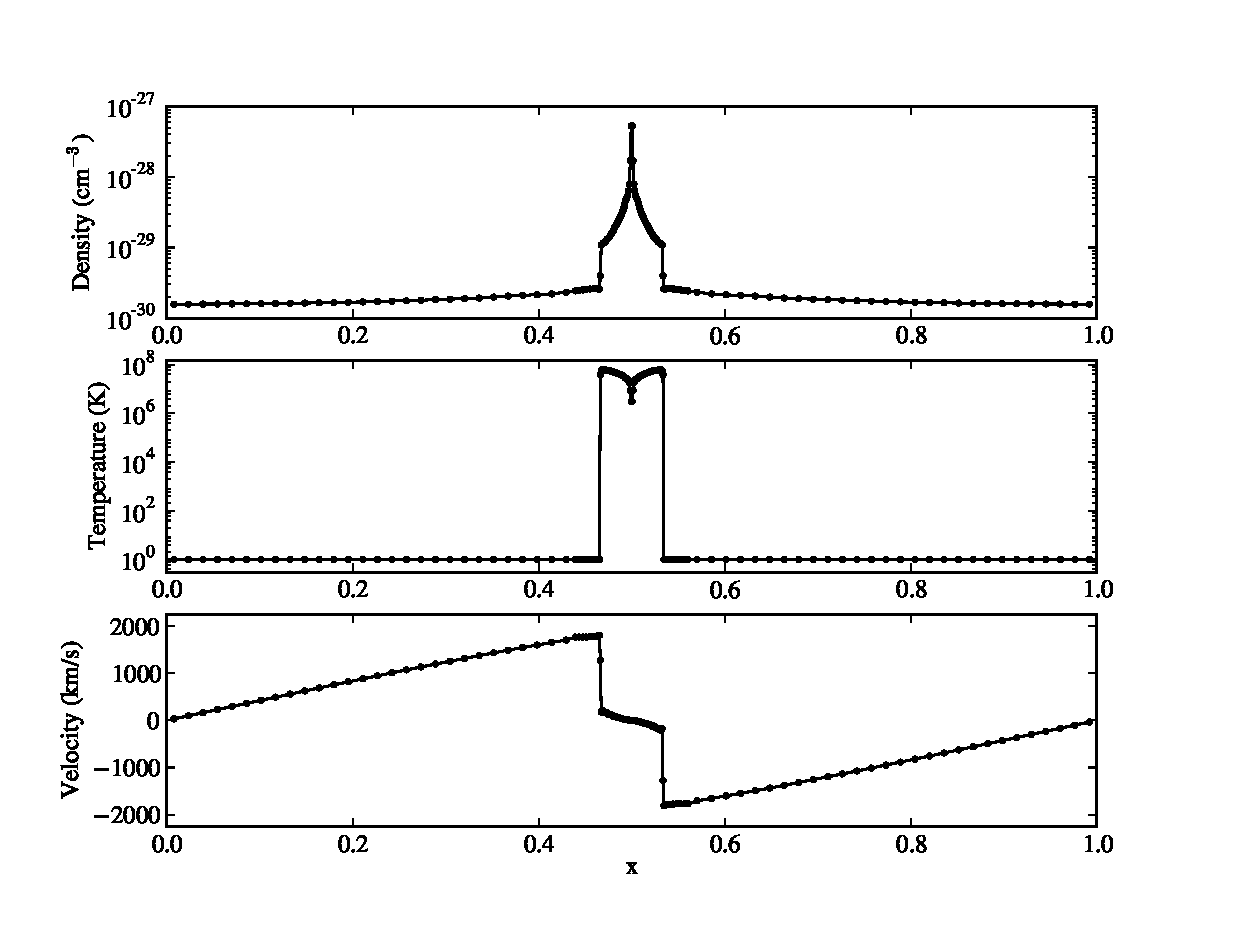
\includegraphics[width=0.8\textwidth]{figures/AMRZeldovichPancake.eps}
\caption{Zel`Dovich Pancake test shown at z$ = 0$, initialized in a
$\Omega_m = 1$ universe at z$ = 20$ on a one-dimensional grid having
64 cells, and further refined by factors of four based on cell mass
and the presence of shocks for up to two additional levels of mesh,
having a maximum effective resolution of 1024 grid cells.}
\label{fig.pancake}
\end{center}
\end{figure}


%%%%%%%%%%%%%%%%%%%%%%%%%%%%%%%%%%%%%%%
\subsubsection{MHD: Orszag-Tang Vortex}
\label{sec.tests.mhd}
Figure \ref{fig.orszag} shows the Orszag-Tang vortex problem, a
typical test problem for MHD \citep{Orszag79}.  The left panel shows
the MHD-CT result, while the right panel shows the Dedner result.
This test shows that small scale structure can be generated in MHD
from large scale initial perturbations.  The test begins with uniform
density, $\rho_0=25/36 \pi$ and pressure, $P_0=5/12 \pi$.  There is a
single rotational mode in the velocity, and two in the magnetic field:
${\bf v}_0 $ = (-sin(2$\pi$ y) $ \hat{x}$ , sin(2$\pi$ x) $\hat{y}$),
${\bf B}_0$ = (-sin(2 $\pi$ y) $ \hat{x},$ sin( 4 $\pi$ x )$\hat{y}$).
The simulation is evolved to t=0.48.  One can see that the structures
are accurately represented as compared to, for instance,
\citet{Toth00}, and that the resolution of shocks is comparable in
both methods.

{\emph Dave's note: I'll probably play around with these results in
future versions.}

\begin{figure}
\begin{center}
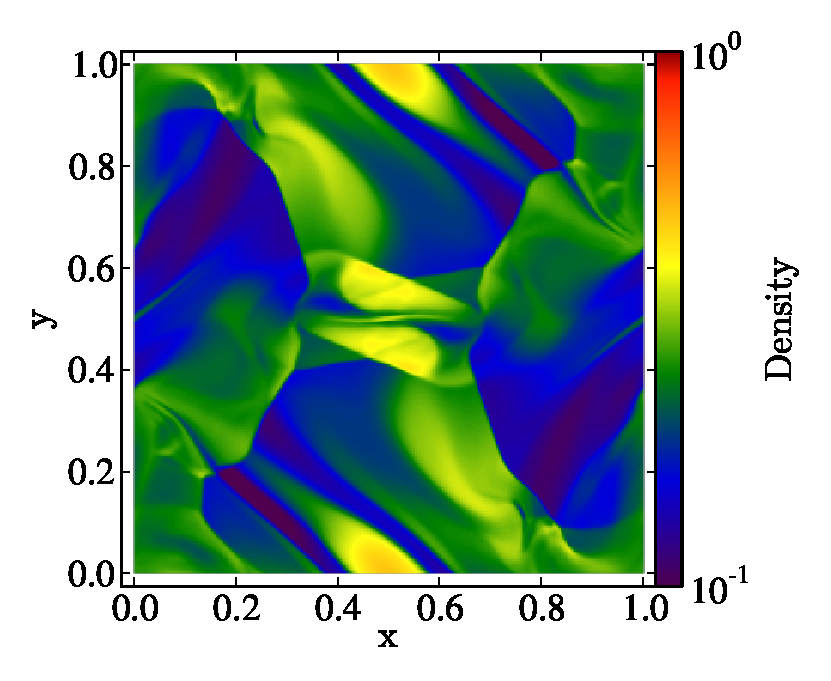
\includegraphics[width=0.4\textwidth]{figures/MHDCT_OrszagTang_Density.eps}
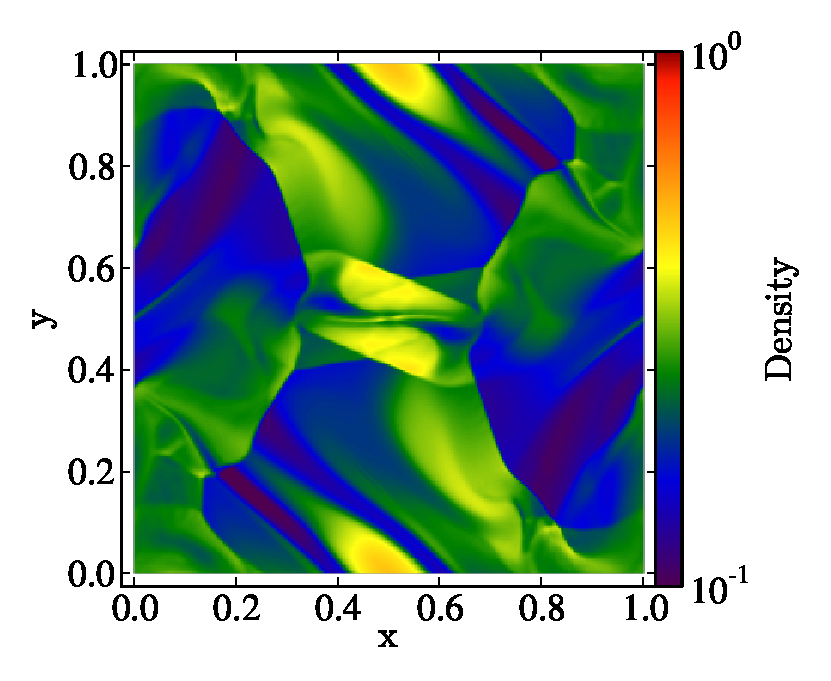
\includegraphics[width=0.4\textwidth]{figures/MHDDedner_OrszagTang_Density.eps}
\caption{TANG}
\label{fig.orszag}
\end{center}
\end{figure}


%%%%%%%%%%%%%%%%%%%%%%%%%%%%%%%%%%%%%%%
\subsubsection{One-zone collapse test}
\label{sec.tests.1-zone}
The one-zone collapse test simulates the collapse of a
self-gravitating gas cloud using a semi-analytic model for the
evolution of gas density and adiabatic heat input as a function of
time.  It is designed to test the chemistry and cooling modules over a
wide range in densities and over physically motivated timescales.
Because this test disables the hydrodynamic and gravity solvers and
uses a simple model for the density evolution, it is far faster than
running a true collapse simulation.  The density evolution is based on
the self-similar Larson-Penston \citep{1969MNRAS.145..271L,
  1969MNRAS.144..425P} solution for isothermal collapse with a
modification to account for the efficiency with which the heat
introduced by compression can be radiated away
\citep{1983ApJ...265.1047Y}.  Our implementation, described briefly
here, follows the work of \citet{2005ApJ...626..627O}, which one
should consult for further details.  The density evolution is given by 
\begin{equation}
\frac{d\rho}{dt} = \frac{\rho}{t_{col}},
\end{equation}
where the collapse timescale, $t_{col}$, is
\begin{equation} \label{eqn.tcol}
t_{col} = \frac{t_{dyn}}{\sqrt{1 - f}},
\end{equation}
and $t_{dyn}$ is the dynamical time, expressed as
\begin{equation}
t_{dyn} = \sqrt{\frac{3 \pi}{32 G \rho}}.
\end{equation}
The collapse timescale is altered from the dynamical time by the
factor, $f$ in Equation \ref{eqn.tcol}, which an approximation of the
ratio of the pressure to the force of gravity.  The value of $f$
depends on the effective adiabatic index, $\gamma_{ef} \equiv (\partial
ln\ p / \partial ln\ \rho)$, which we calculate by linearly extrapolating
from derivative values for the two previous timesteps.  For the value
of $f$, we use the piecewise function of \citet{2005ApJ...626..627O},
given by
\begin{equation}
f = \left\{
  \begin{array}{ll}
  0, & \gamma_{ef} < 0.83,\\
  0.6 + 2.5 (\gamma_{ef} - 1) - 6.0 (\gamma_{ef} - 1)^{2}, & 0.83 <
  \gamma_{ef} < 1,\\
  1.0 + 0.2 (\gamma_{ef} - 4/3) - 2.9 (\gamma_{ef} - 4/3)^{2}, & \gamma_{ef} > 1.
\end{array} \right.
\end{equation}
The specific energy evolves as
\begin{equation}
\frac{de}{dt} = -p \frac{d}{dt} \frac{1}{\rho} - \Lambda,
\end{equation}
where $\Lambda$ is the cooling rate in units of erg s$^{-1}$ g$^{-1}$
and energy, temperature, density, and pressure are related by the
ideal gas law.  Figure \ref{fig.onezone} shows an example of the
one-zone collapse test performed with an initial number density of 1
cm$^{-3}$ and temperature of 100 K using the 12 species chemistry
network with H, D, and He species and metal cooling rates calculated
with Cloudy.

\begin{figure}
  \begin{center}
    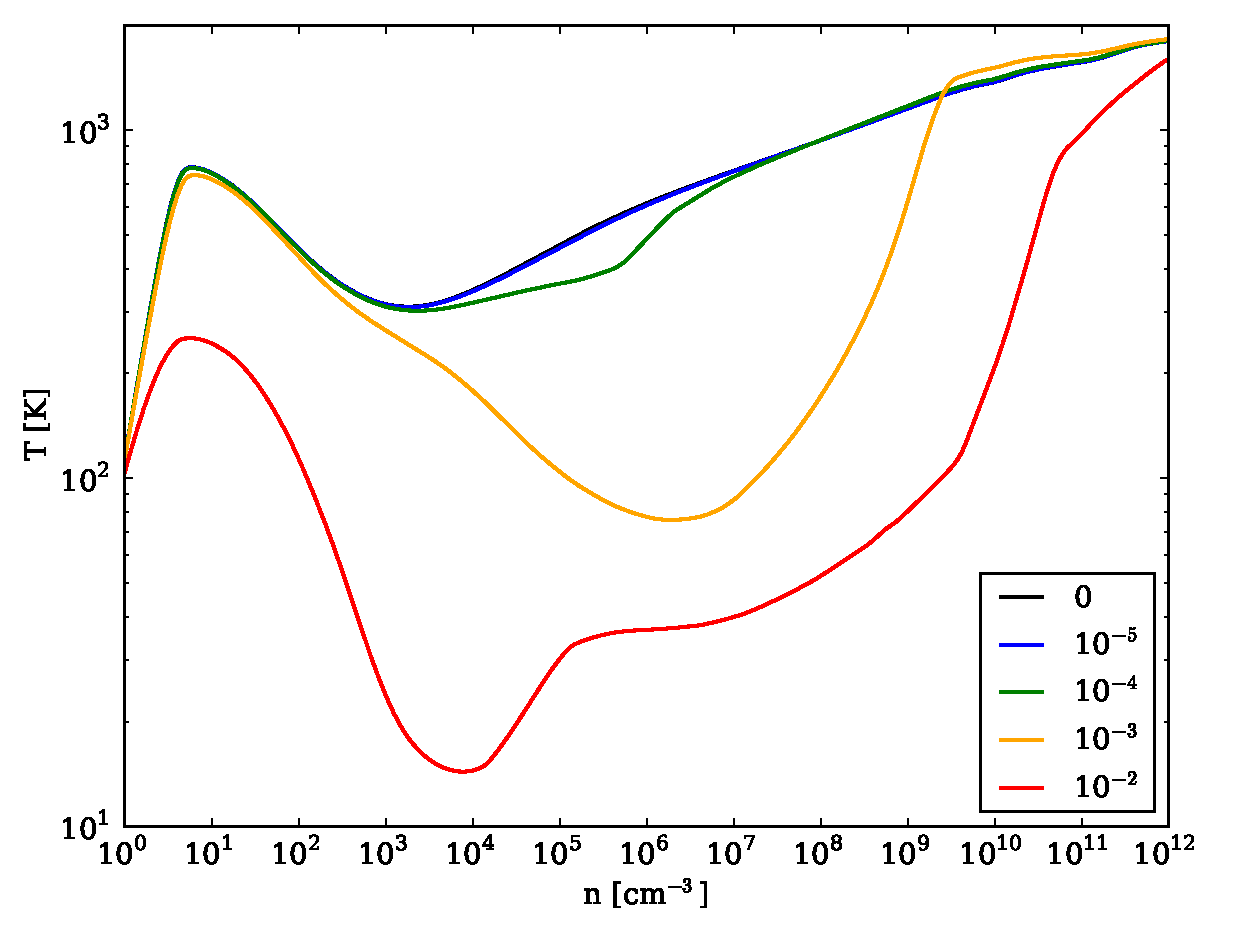
\includegraphics[width=1.0\textwidth]{figures/OneZoneCollapseTest.eps}
  \end{center}
  \caption{Evolution of temperature versus number density for a one-zone
    collapse test for gas at metallicities from 0 to 10$^{-2} Z_{\odot}$
    using the primordial chemistry network with tabulated metal cooling
    rates calculated with Cloudy.}
  \label{fig.onezone}
\end{figure}


%%%%%%%%%%%%%%%%%%%%%%%%%%%%%%%%%%%%%%%
\subsubsection{Photo-evaporation of a dense clump}
\label{sec.tests.raytracing}

The photo-evaporation of dense clumps is prevalent in radiation
hydrodynamics simulations, and this test problem examines the
ionization front propagation into the dense clump, shadowing effects
behind the clump, and the hydrodynamic response on the clump from
photo-heating.  The problem setup is the same as Test 7 in the
Cosmological Radiative Transfer Comparison Project
\citep{IlievEtAl2009} and \citet{Wise11_Moray}.  The simulation domain
is 6.6~kpc on a side with an ambient medium of pure neutral hydrogen
$n_{\rm H} = 2 \times 10^{-4}\; \cubecm$ and $T = 8000 \unit{K}$.  We
place a spherical overdensity in hydrostatic equilibrium with the
ambient medium.  It has a radius $r = 0.8 \unit{kpc}$, hydrogen
density $n_{\rm H} = 0.04 \cubecm$, and temperature $T = 40$ K, and it
is centered at $(x,y,z) = (5, 3.3, 3.3) \unit{kpc}$.  In
\citet{IlievEtAl2009}, all of the codes used a fixed $128^3$ grid to
ease the comparison, but in this test to demonstrate a higher
resolution AMR solution, we employ a $128^3$ grid with two additional
levels of refinement with cells with a baryon mass (method 2 in
\S\ref{sec:refinement_criteria}) greater than 1.5 being flagged for
refinement.  This test is run for 15 Myr.

This cloud is subject to radiation from a point source at the center
of the $y=0$ boundary with an ionizing photon luminosity
$\dot{N}_\gamma = 3 \times 10^{51}$ photons s$^{-1}$, corresponding to
a flux $F_0 = 10^6 \unit{photons s}^{-1} \unit{cm}^{-2}$ at the clump
surface closest to the radiation source.  The radiation source has a
spectrum of a $T = 10^5 \unit{K}$ blackbody, and we use four energy
groups with the following mean energies and relative luminosities:
$E_i = (17.98, 31.15, 49.09, 76.98) \unit{eV}, L_i/L = (0.23, 0.36,
0.24, 0.06)$ that are optimized to reduce errors in the solutions with
a full spectrum and energy discretization \citep{Mirocha12}.  Note
that this choice of energy groups is different from
\citet{Wise11_Moray}.  We use a minimum angular resolution of 10 rays
per cell and a constant radiative transfer timestep of 25 kyr.  Figure
\ref{fig:shadowing} depicts the clump after at $t = 15$ Myr with the
outer layers expanding after being photo-heated.  It also shows the
sharp shadowing effects of the dense clump in the neutral fraction
plot that is representative of ray tracing techniques.

\begin{figure}
  \centering
  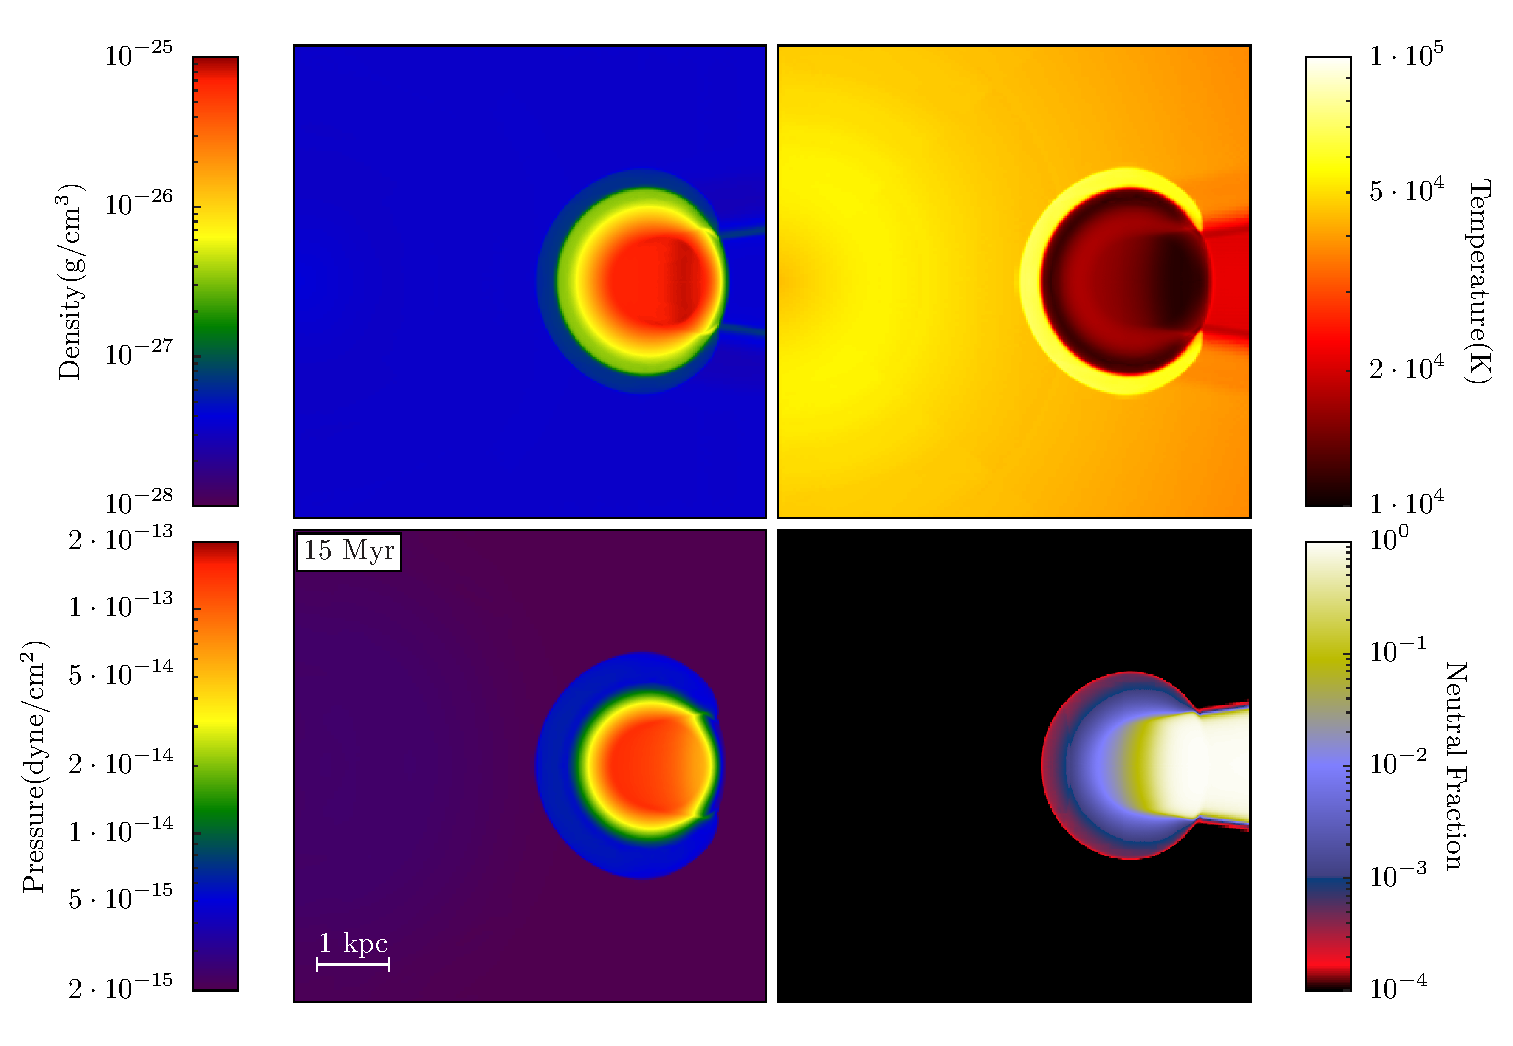
\includegraphics[width=1.0\textwidth]{figures/code-test-shadowing.eps}
  \caption{Photo-evaporation of a dense clump.  Clockwise from the
    upper left-hand side: slices through the clump center of the
    density, temperature, neutral fraction, and pressure.}
  \label{fig:shadowing}
\end{figure}

%%%%%%%%%%%%%%%%%%%%%%%%%%%%%%%%%%%%%%%
\subsubsection{Representative FLD test}
\label{sec.tests.fld}

\red{(Dan)}
One test for the implicit FLD: best/hardest one.



%%%%%%%%%%%%%%%%%%%%%%%%%%%%%%%%%%%%%%%

\subsubsection{Representative thermal conduction test}
\label{sec.tests.conduct}
\red{(Brian)}
One test for the thermal conduction (maybe 1 for isotropic, 1 for
anisotropic).  Figure~\ref{fig.conduct}.

\begin{figure}
\begin{center}
\includegraphics[width=0.4\textwidth]{figures/iso_conduction_final_output.eps}
\includegraphics[width=0.4\textwidth]{figures/aniso_conduction_final_output.eps}
\caption{Temperature blah blah.  Conduction tests!}
\label{fig.conduct}
\end{center}
\end{figure}


%%% Local Variables: 
%%% mode: latex
%%% TeX-master: "ms"
%%% End: 
